\documentclass{beamer}
\usetheme{ttuStatsCamp}
\usefonttheme{serif}
\usepackage[T1]{fontenc}
\usepackage[utf8]{inputenc}
\usepackage{url}
\usepackage{graphicx}
\usepackage{setspace}
\usepackage[natbibapa]{apacite}
\usepackage{color}
\usepackage{amsmath}
\usepackage{amsfonts}
\usepackage{Sweavel}
\usepackage{listings}
\usepackage{fancybox}

\def\Sweavesize{\scriptsize}
\def\Rcolor{\color{black}}
%\def\Routcolor{\color{red}}
\def\Rcommentcolor{\color{violet}}
\def\Rbackground{\color[gray]{0.85}}
\def\Routbackground{\color[gray]{0.85}}

\lstset{tabsize=2, breaklines=true, style=Rstyle}



\newcommand{\red}[0]{\textcolor{red}}
\newcommand{\green}[0]{\textcolor{green}}
\newcommand{\blue}[0]{\textcolor{blue}}
\newcommand{\comment}[1]{}
\newcommand{\va}[0]{\vspace{12pt}}
\newcommand{\vb}[0]{\vspace{6pt}}
\newcommand{\vc}[0]{\vspace{3pt}}
\newcommand{\vx}[1]{\vspace{#1pt}}

\title[Lecture 7]{Lecture 7: Basic Moderation}

\author{Kyle M. Lang}

\institute[TTU IMMAP]{
  Institute for Measurement, Methodology, Analysis \& Policy\\
  Texas Tech University\\
  Lubbock, TX
}

\date{2016 Stats Camp}

\setbeamertemplate{frametitle continuation}{}

\begin{document}

\setkeys{Gin}{width=\textwidth}

\input{sweaveFiles/-001}


\begin{frame}[plain]
  
  \titlepage
  
\end{frame}


\begin{frame}{Outline}

  \begin{itemize}
  \item Review the moderation hypothesis
    \va
  \item Doing basic moderation analysis
    \va
  \item Visualizing the moderation (a little)
    \va
  \item Probing the moderation (also a little)
  \end{itemize}

\end{frame}



\begin{frame}{Intuition}

  So far we've been discussing \emph{mediation}
  \vb
  \begin{itemize}
  \item Mediation allows us to ask \emph{how} one variable ($X$)
    affects another variable ($Y$).
    \vc
    \begin{itemize}
    \item Namely, through the intermediary influence of a third
      variable ($M$).
    \end{itemize}
  \end{itemize}
  \va
  Now, we're stepping into the realm of \emph{moderation}
  \vb
  \begin{itemize}
  \item Moderation allows us to ask \emph{when} one variable ($X$) affects
    another variable ($Y$).
    \vc
    \begin{itemize}
    \item Here, we're considering the effect of $X$ on $Y$
      conditional on certain levels of a third variable $Z$.
    \end{itemize}
  \end{itemize}

\end{frame}



\begin{frame}{Conceptual Diagram}

  We can diagrammatically represent the above intuition with:

  \begin{figure}
    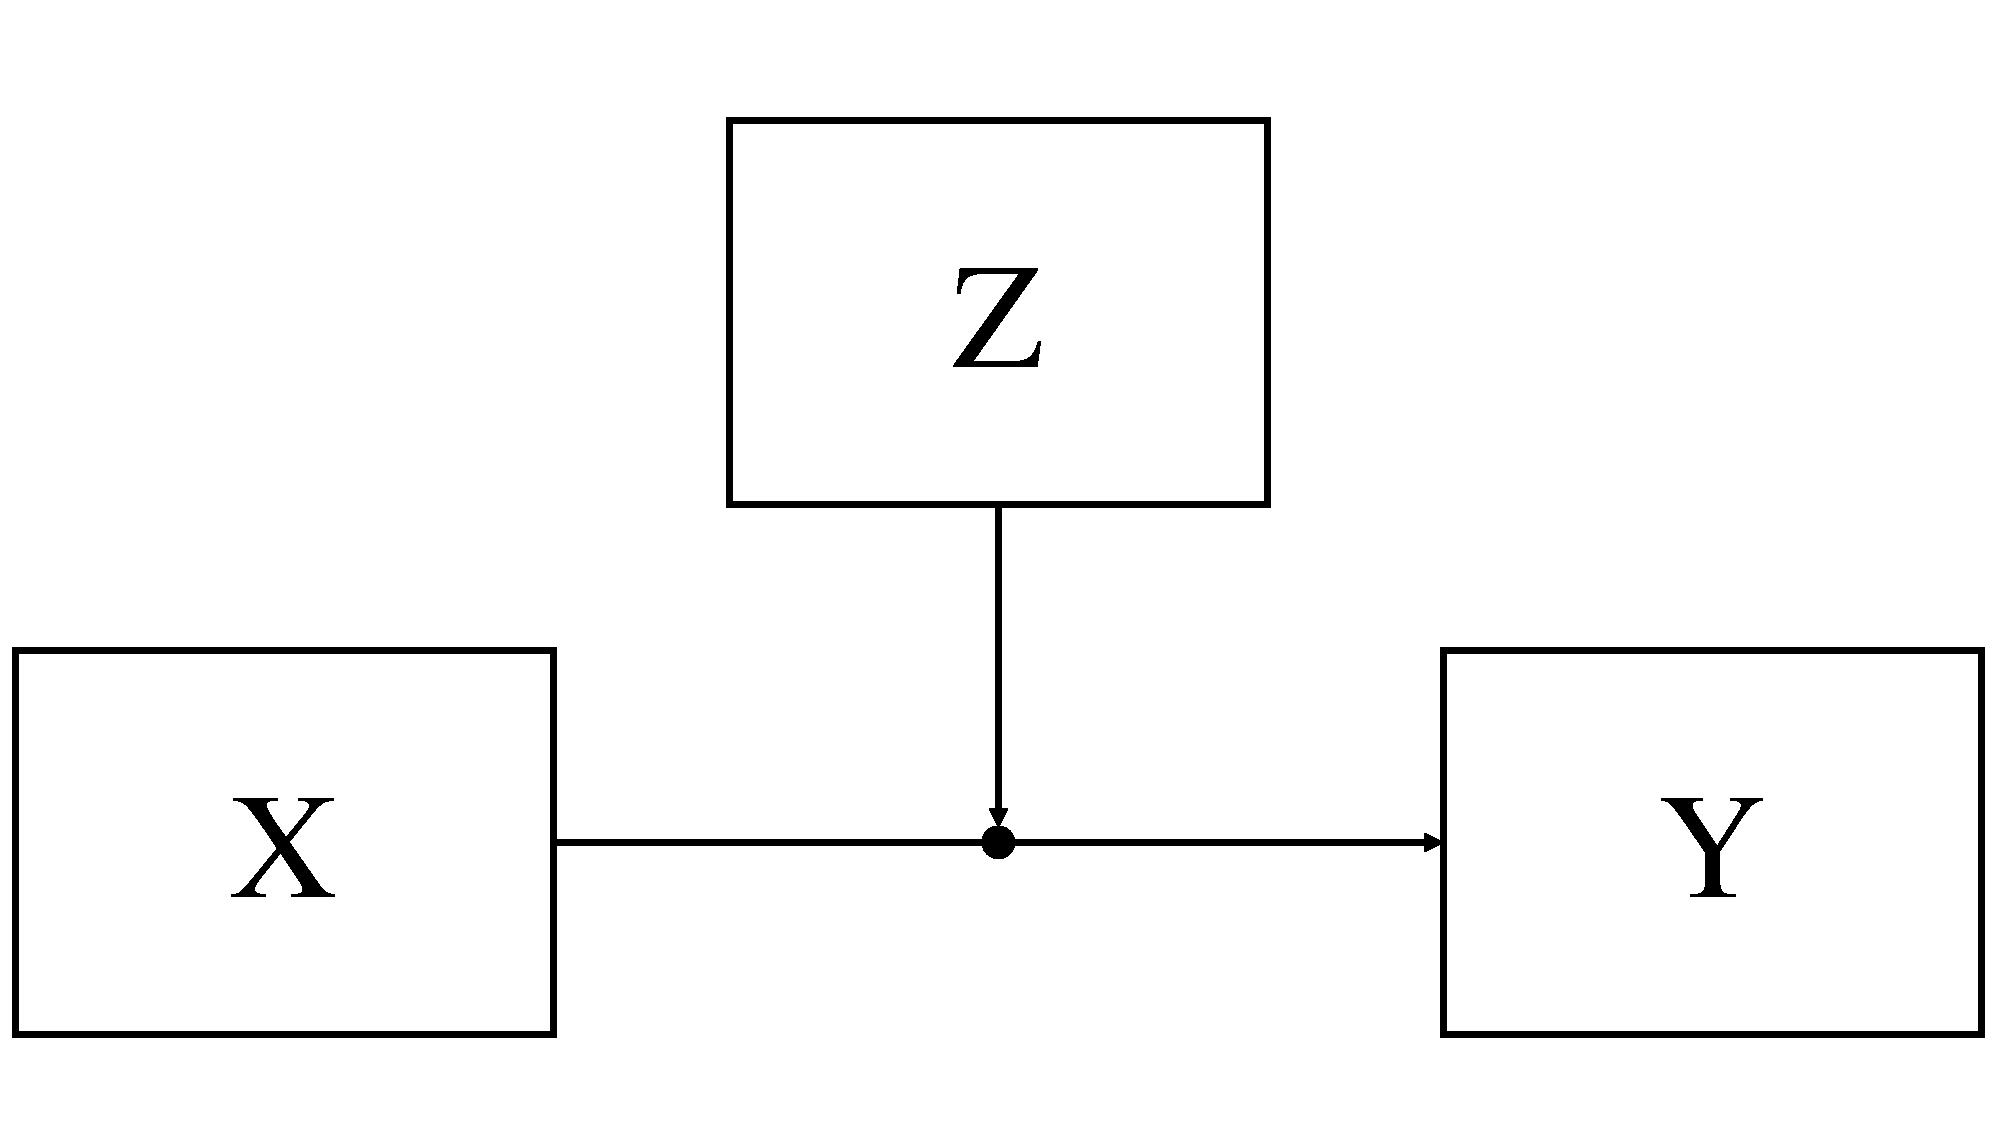
\includegraphics[width=\textwidth]{figures/modConcept.pdf}
  \end{figure}

\end{frame}



\begin{frame}{Equations}

  In simple additive MLR, we might have the following equation:
  \begin{align}
    Y = \alpha + \beta_1X + \beta_2Z + e_i \label{additiveEq}
  \end{align}
  This additive equation assumes that $X$ and $Z$ are independent
  predictors of $Y$.\\
  \va
  When $X$ and $Z$ are independent predictors, the following
  points are true:
  \vb
  \begin{itemize}
  \item $X$ and $Z$ \emph{can} be correlated
    \vb
  \item $\beta_1$ and $\beta_2$ are \emph{partial} regression
    coefficients
    \vb
  \item \red{The effect of $X$ on $Y$ is the same at \textbf{all levels} of
    $Z$, and the effect of $Z$ on $Y$ is the same at \textbf{all
      levels} of $X$}
  \end{itemize}

\end{frame}



\begin{frame}{Equations}

  When testing moderation, we hypothesize that the effect of $X$ on
  $Y$ in Equation \ref{additiveEq} varies as a function of $Z$.\\
  \va
  We can represent this concept with the following equation:
  \begin{align}
    Y = \alpha + f(Z)X + \beta_2Z + e_i
  \end{align}
  \pause
  If we assume that $Z$ linearly affects the relationship between $X$
  and $Y$, then we can take:
  \begin{align}
    f(Z) = \beta_1 + \beta_3Z
  \end{align}
  \pause
  Which, after substitution, leads to:
  \begin{align}
    Y = \alpha + (\beta_1 + \beta_3Z)X + \beta_2Z + e_i
  \end{align}
  \pause
  Which, after distributing $X$ and reordering terms, becomes:
  \begin{align}
    Y = \alpha + \beta_1X + \beta_2Z + \beta_3XZ + e_i
  \end{align}

\end{frame}


\begin{frame}{Analytical Model}

  We can diagrammatically represent the analytical model we'll actually
  be fitting with:

  \begin{figure}
    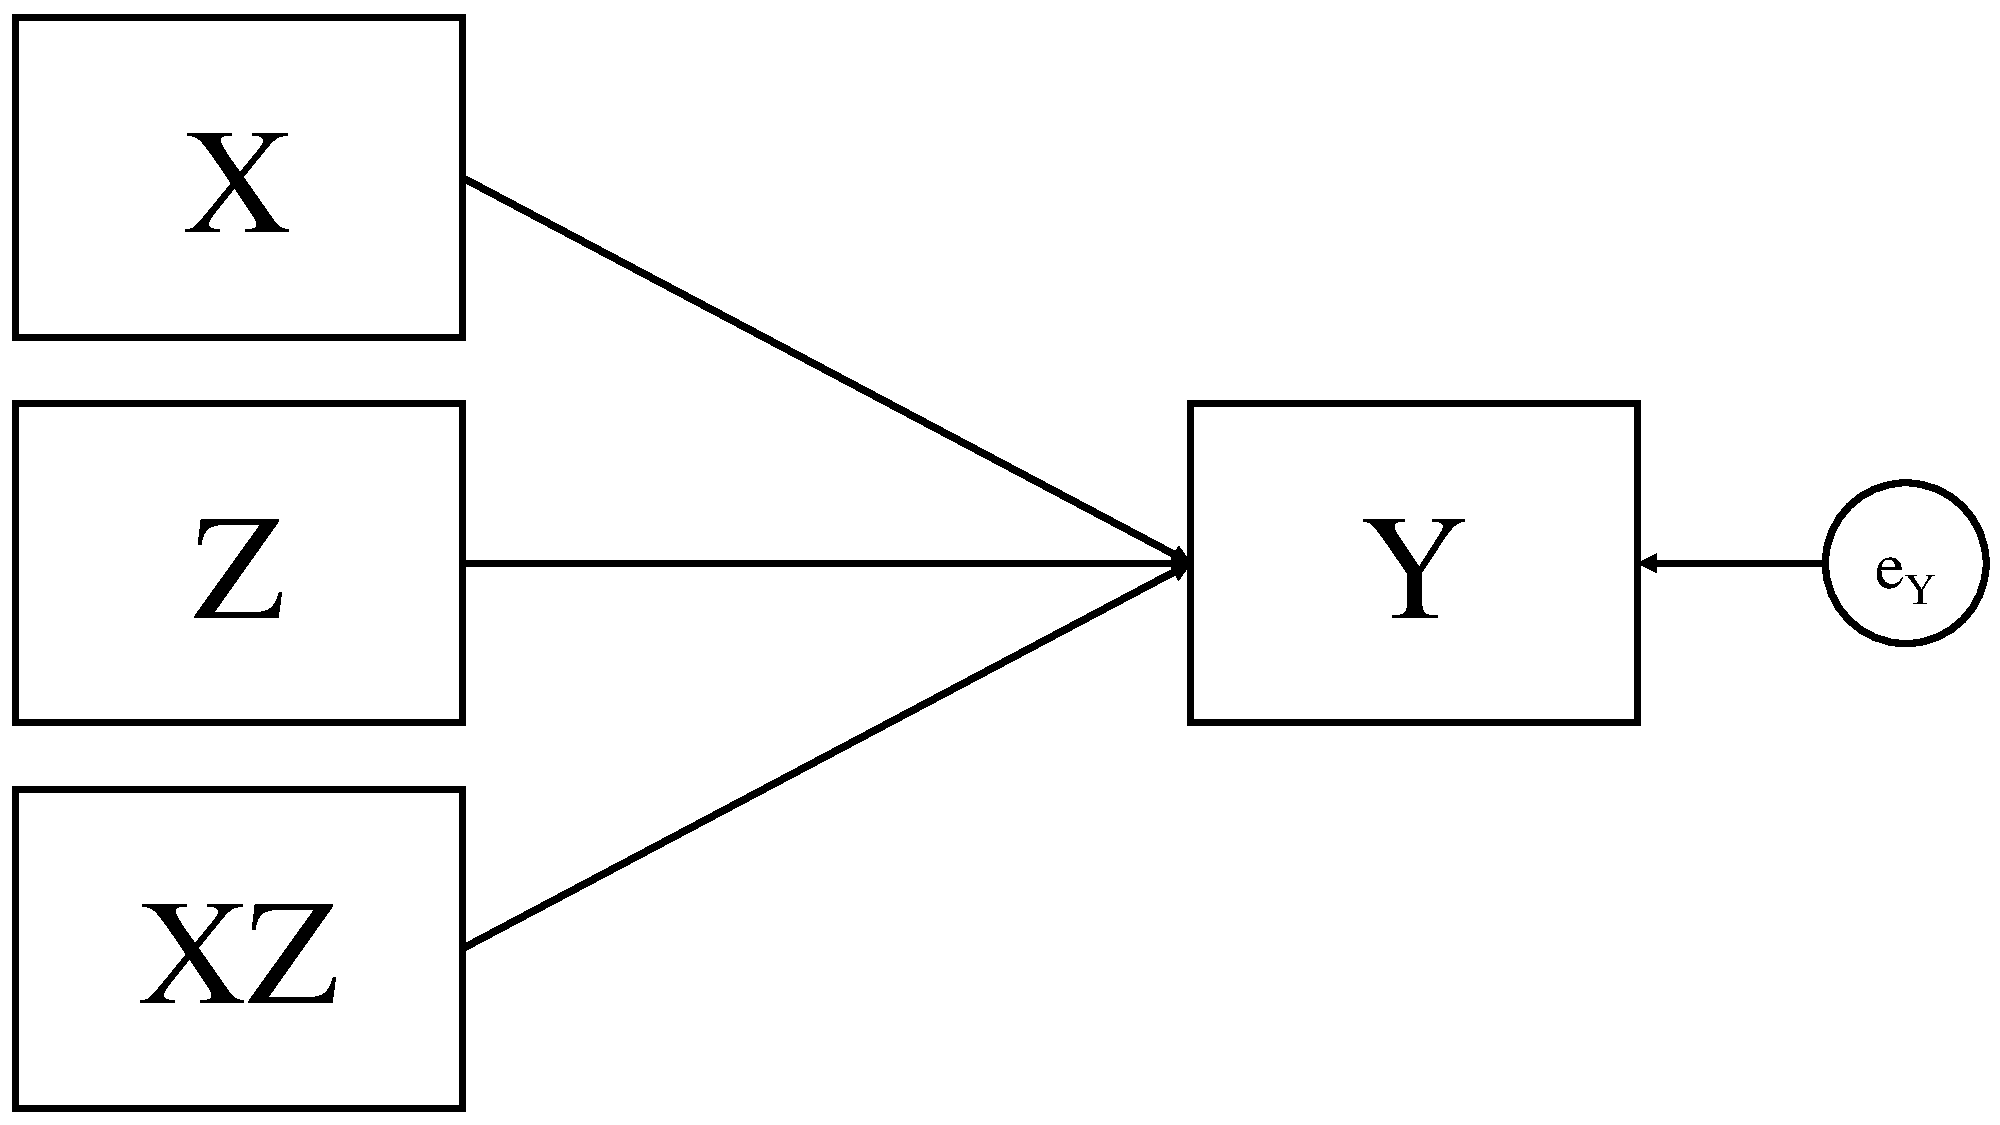
\includegraphics[width=\textwidth]{figures/modAnalytic.pdf}
  \end{figure}

\end{frame}


\begin{frame}{Analytical Model}

  By adding the appropriate path labels, we get:

  \begin{figure}
    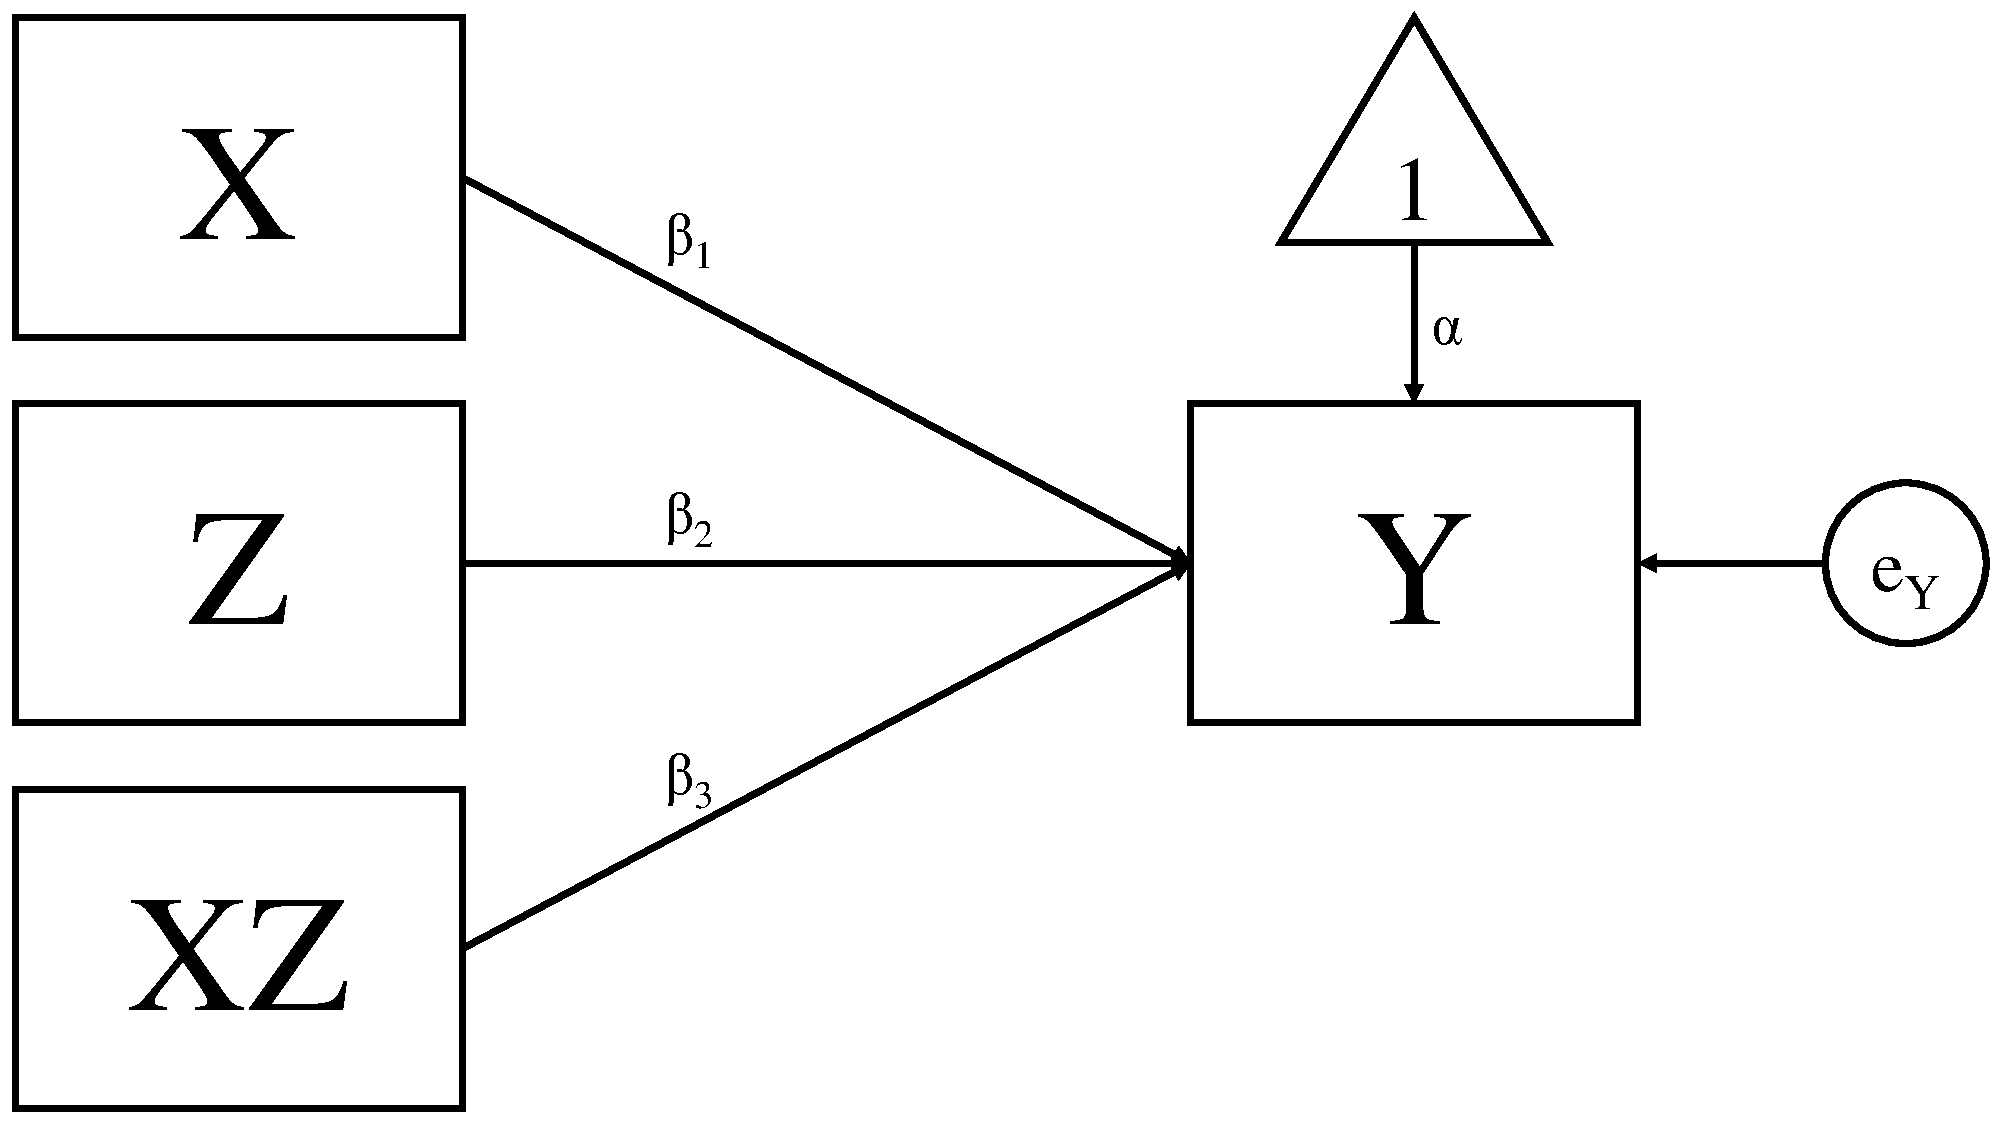
\includegraphics[width=\textwidth]{figures/modAnalytic2.pdf}
  \end{figure}

\end{frame}

\begin{frame}{Testing Moderation}

  This is the equation we'll be working with:\\
  \begin{center}\ovalbox{$Y = \alpha + \beta_1X + \beta_2Z + \beta_3XZ + e_i$}\end{center}
  \va
  Or, after fitting the above to some data:
  \begin{center}\ovalbox{$\hat{Y} = \hat{\alpha} + \hat{\beta}_1X + \hat{\beta}_2Z + \hat{\beta}_3XZ$}\end{center}
  \va
  To test for significant moderation, we simply need to see if
  $\hat{\beta}_3$ is significantly different from zero.\\
  \va
  We do so using simple linear regression modeling.

\end{frame}



\begin{frame}{Example}

Data from the \emph{National Longitudinal Survey of Youth}\\
\va
We suspect that participants' weight to height ratio is predictive of
their levels of depression.\\
\va
We further suspect that this effect may be differentially expressed
depending on how the participants perceive their own weight.

\end{frame}


\begin{frame}{Example}

  This is the conceptual diagram for the model we'll fit:

  \begin{figure}
    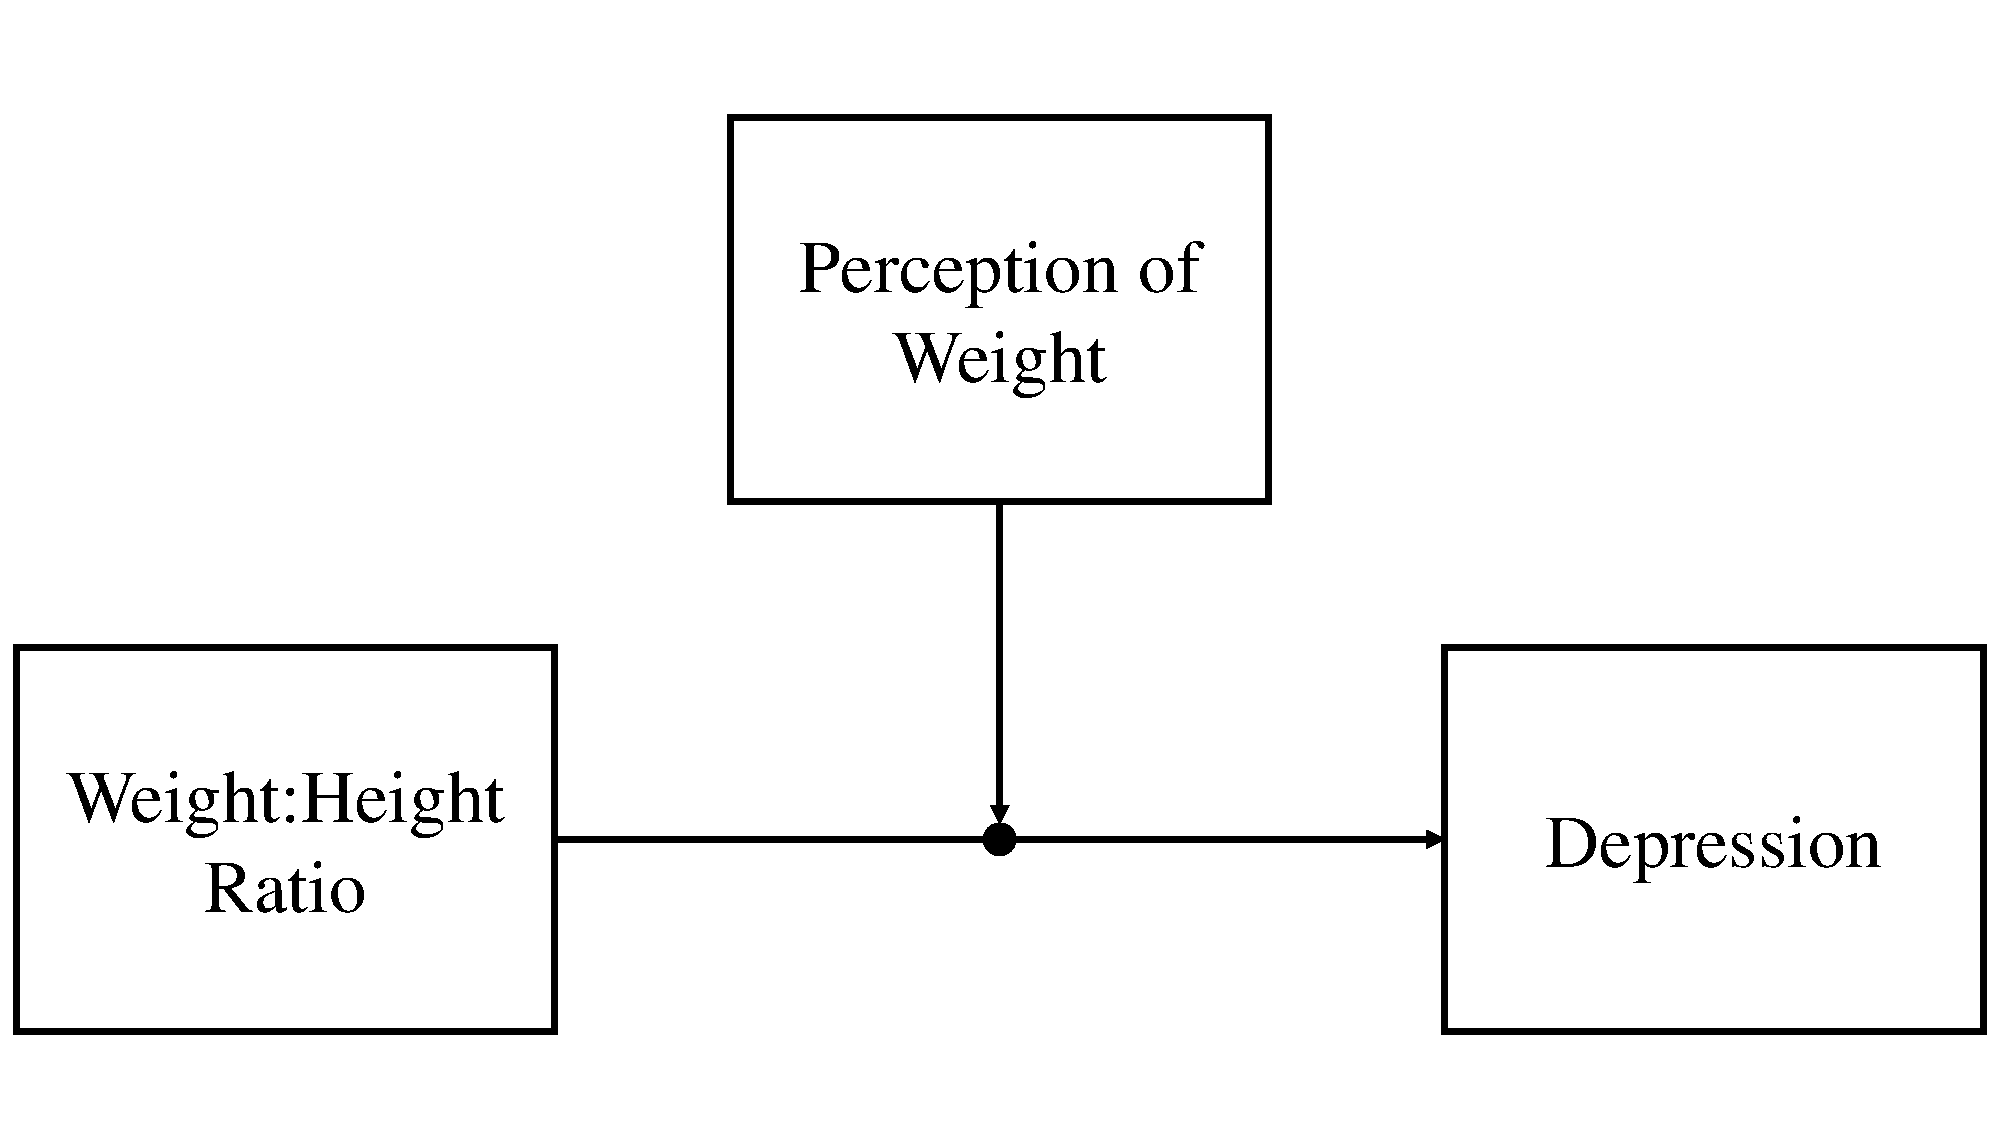
\includegraphics[width=\textwidth]{figures/modExample1.pdf}
  \end{figure}

\end{frame}


\begin{frame}[allowframebreaks]{Example}

\begin{Schunk}
\begin{Sinput}
 library(lavaan)
 dataDir <- "../data/"
 dat1 <- readRDS(paste0(dataDir, "adamsKlpsData.rds"))
 ## Specify the CFA model:
 mod1.1 <- "
 merit =~ meritP1 + meritP2 + meritP3
 policy =~ policyP1 + policyP2 + policyP3
 "
 ## Fit the CFA and check model:
 out1.1 <- cfa(mod1.1, data = dat1, std.lv = TRUE)
 ## Check model fit:
 round(fitMeasures(out1.1)[c("chisq", "df", "pvalue", "cfi", 
                             "tli", "rmsea", "srmr")], 4)
\end{Sinput}
\begin{Soutput}
  chisq      df  pvalue     cfi     tli   rmsea    srmr 
16.8695  8.0000  0.0315  0.9215  0.8529  0.1129  0.0653 
\end{Soutput}
\begin{Sinput}
 summary(out1.1)
\end{Sinput}
\begin{Soutput}
lavaan (0.5-20) converged normally after  22 iterations

  Number of observations                            87

  Estimator                                         ML
  Minimum Function Test Statistic               16.869
  Degrees of freedom                                 8
  P-value (Chi-square)                           0.031

Parameter Estimates:

  Information                                 Expected
  Standard Errors                             Standard

Latent Variables:
                   Estimate  Std.Err  Z-value  P(>|z|)
  merit =~                                            
    meritP1           0.690    0.134    5.155    0.000
    meritP2           0.968    0.142    6.830    0.000
    meritP3           0.748    0.137    5.458    0.000
  policy =~                                           
    policyP1          0.851    0.186    4.570    0.000
    policyP2          0.996    0.167    5.967    0.000
    policyP3          1.121    0.177    6.339    0.000

Covariances:
                   Estimate  Std.Err  Z-value  P(>|z|)
  merit ~~                                            
    policy           -0.336    0.131   -2.563    0.010

Variances:
                   Estimate  Std.Err  Z-value  P(>|z|)
    meritP1           0.865    0.165    5.248    0.000
    meritP2           0.445    0.201    2.211    0.027
    meritP3           0.833    0.172    4.857    0.000
    policyP1          1.836    0.324    5.671    0.000
    policyP2          0.942    0.256    3.683    0.000
    policyP3          0.857    0.297    2.882    0.004
    merit             1.000                           
    policy            1.000                           
\end{Soutput}
\end{Schunk}


\begin{Schunk}
\begin{Sinput}
 round(fitMeasures(out1)[c("chisq", "df", "pvalue", "cfi", 
                           "tli", "rmsea", "srmr")], 3)
\end{Sinput}
\begin{Soutput}
 chisq     df pvalue    cfi    tli  rmsea   srmr 
41.021 24.000  0.017  0.987  0.981  0.038  0.026 
\end{Soutput}
\end{Schunk}

\pagebreak
\begin{Schunk}
\begin{Sinput}
 mod3 <- "
 att3 ~ att2 + b2*conf2 + cp2*horn2
 att2 ~ att1 + b1*conf1 + cp1*horn1
 
 conf3 ~ conf2 + a2*horn2
 conf2 ~ conf1 + a1*horn1
 
 horn3 ~ horn2
 horn2 ~ horn1
 
 horn3 ~~ conf3 + att3
 conf3 ~~ att3
 
 horn2 ~~ conf2 + att2
 conf2 ~~ att2
 
 a1 == a2
 b1 == b2
 cp1 == cp2
 "
 out3 <- sem(mod3, data = dat1)
 summary(out3)
\end{Sinput}
\begin{Soutput}
lavaan (0.5-20) converged normally after  46 iterations

  Number of observations                           500

  Estimator                                         ML
  Minimum Function Test Statistic              294.220
  Degrees of freedom                                18
  P-value (Chi-square)                           0.000

Parameter Estimates:

  Information                                 Expected
  Standard Errors                             Standard

Regressions:
                   Estimate  Std.Err  Z-value  P(>|z|)
  att3 ~                                              
    att2              0.497    0.035   14.234    0.000
    conf2     (b2)    0.098    0.019    5.200    0.000
    horn2    (cp2)    0.083    0.072    1.157    0.247
  att2 ~                                              
    att1              0.530    0.040   13.345    0.000
    conf1     (b1)    0.098    0.019    5.200    0.000
    horn1    (cp1)    0.083    0.072    1.157    0.247
  conf3 ~                                             
    conf2             0.684    0.035   19.602    0.000
    horn2     (a2)    0.493    0.107    4.596    0.000
  conf2 ~                                             
    conf1             0.623    0.032   19.546    0.000
    horn1     (a1)    0.493    0.107    4.596    0.000
  horn3 ~                                             
    horn2             0.826    0.030   27.609    0.000
  horn2 ~                                             
    horn1             0.714    0.024   29.181    0.000

Covariances:
                   Estimate  Std.Err  Z-value  P(>|z|)
  conf3 ~~                                            
    horn3             1.016    0.155    6.556    0.000
  att3 ~~                                             
    horn3             0.322    0.093    3.483    0.000
    conf3             3.574    0.465    7.691    0.000
  conf2 ~~                                            
    horn2             0.836    0.124    6.721    0.000
  att2 ~~                                             
    horn2             0.273    0.083    3.289    0.001
    conf2             2.027    0.400    5.067    0.000

Variances:
                   Estimate  Std.Err  Z-value  P(>|z|)
    att3              6.019    0.381   15.811    0.000
    att2              6.041    0.382   15.811    0.000
    conf3            15.814    1.000   15.811    0.000
    conf2            12.570    0.795   15.811    0.000
    horn3             0.695    0.044   15.811    0.000
    horn2             0.560    0.035   15.811    0.000

Constraints:
                                               |Slack|
    a1 - (a2)                                    0.000
    b1 - (b2)                                    0.000
    cp1 - (cp2)                                  0.000
\end{Soutput}
\begin{Sinput}
 chiDiff <- fitMeasures(out3)["chisq"] -
     fitMeasures(out1)["chisq"]
 dfDiff <- fitMeasures(out3)["df"] -
     fitMeasures(out1)["df"]
 pchisq(chiDiff, dfDiff, lower = FALSE)
\end{Sinput}
\begin{Soutput}
     chisq 
0.02684148 
\end{Soutput}
\end{Schunk}

\pagebreak
\begin{Schunk}
\begin{Sinput}
 mod4 <- "
 att3 ~ att2 + b2*conf2 + cp*horn1
 att2 ~ att1 + b1*conf1
 
 conf3 ~ conf2 + a2*horn2
 conf2 ~ conf1 + a1*horn1
 
 att2 + att3 ~ income
 conf2 + conf3 ~ income 
 horn2 + horn3 ~ income
 
 horn3 ~ horn2
 horn2 ~ horn1
 
 horn3 ~~ conf3 + att3
 conf3 ~~ att3
 
 horn2 ~~ conf2 + att2
 conf2 ~~ att2
 
 ab := a1*b2
 "
 out4 <- sem(mod4, data = dat1, se = "boot", boot = nBoot)
 summary(out4)
\end{Sinput}
\begin{Soutput}
lavaan (0.5-20) converged normally after  63 iterations

  Number of observations                           500

  Estimator                                         ML
  Minimum Function Test Statistic              219.789
  Degrees of freedom                                16
  P-value (Chi-square)                           0.000

Parameter Estimates:

  Information                                 Observed
  Standard Errors                            Bootstrap
  Number of requested bootstrap draws             2000
  Number of successful bootstrap draws            2000

Regressions:
                   Estimate  Std.Err  Z-value  P(>|z|)
  att3 ~                                              
    att2              0.513    0.039   13.099    0.000
    conf2     (b2)    0.022    0.027    0.826    0.409
    horn1     (cp)   -0.119    0.084   -1.418    0.156
  att2 ~                                              
    att1              0.477    0.043   10.980    0.000
    conf1     (b1)    0.084    0.028    3.048    0.002
  conf3 ~                                             
    conf2             0.488    0.041   11.803    0.000
    horn2     (a2)    0.492    0.160    3.076    0.002
  conf2 ~                                             
    conf1             0.543    0.037   14.594    0.000
    horn1     (a1)    0.175    0.146    1.204    0.228
  att2 ~                                              
    income            0.052    0.013    4.108    0.000
  att3 ~                                              
    income            0.057    0.012    4.853    0.000
  conf2 ~                                             
    income            0.110    0.016    6.871    0.000
  conf3 ~                                             
    income            0.148    0.018    8.206    0.000
  horn2 ~                                             
    income            0.016    0.003    5.698    0.000
  horn3 ~                                             
    income            0.013    0.004    3.555    0.000
    horn2             0.780    0.033   23.921    0.000
  horn2 ~                                             
    horn1             0.654    0.026   25.525    0.000

Covariances:
                   Estimate  Std.Err  Z-value  P(>|z|)
  conf3 ~~                                            
    horn3             0.915    0.152    6.020    0.000
  att3 ~~                                             
    horn3             0.322    0.092    3.489    0.000
    conf3             2.971    0.412    7.215    0.000
  conf2 ~~                                            
    horn2             0.678    0.112    6.026    0.000
  att2 ~~                                             
    horn2             0.203    0.083    2.428    0.015
    conf2             1.601    0.382    4.194    0.000

Variances:
                   Estimate  Std.Err  Z-value  P(>|z|)
    att3              5.771    0.351   16.431    0.000
    att2              5.821    0.362   16.099    0.000
    conf3            14.066    0.828   16.988    0.000
    conf2            11.512    0.729   15.792    0.000
    horn2             0.529    0.033   16.004    0.000
    horn3             0.677    0.040   16.788    0.000

Defined Parameters:
                   Estimate  Std.Err  Z-value  P(>|z|)
    ab                0.004    0.007    0.559    0.576
\end{Soutput}
\begin{Sinput}
 parameterEstimates(out4, boot = "bca.simple")[ , -c(1 : 3)]
\end{Sinput}
\begin{Soutput}
   label     est    se      z pvalue ci.lower ci.upper
1          0.513 0.039 13.099  0.000    0.438    0.589
2     b2   0.022 0.027  0.826  0.409   -0.030    0.076
3     cp  -0.119 0.084 -1.418  0.156   -0.275    0.051
4          0.477 0.043 10.980  0.000    0.396    0.565
5     b1   0.084 0.028  3.048  0.002    0.029    0.139
6          0.488 0.041 11.803  0.000    0.410    0.569
7     a2   0.492 0.160  3.076  0.002    0.186    0.818
8          0.543 0.037 14.594  0.000    0.464    0.614
9     a1   0.175 0.146  1.204  0.228   -0.099    0.468
10         0.052 0.013  4.108  0.000    0.028    0.077
11         0.057 0.012  4.853  0.000    0.033    0.079
12         0.110 0.016  6.871  0.000    0.079    0.141
13         0.148 0.018  8.206  0.000    0.114    0.183
14         0.016 0.003  5.698  0.000    0.011    0.022
15         0.013 0.004  3.555  0.000    0.005    0.019
16         0.780 0.033 23.921  0.000    0.714    0.844
17         0.654 0.026 25.525  0.000    0.601    0.703
18         0.915 0.152  6.020  0.000    0.633    1.225
19         0.322 0.092  3.489  0.000    0.143    0.508
20         2.971 0.412  7.215  0.000    2.207    3.834
21         0.678 0.112  6.026  0.000    0.466    0.903
22         0.203 0.083  2.428  0.015    0.040    0.369
23         1.601 0.382  4.194  0.000    0.870    2.387
24         5.771 0.351 16.431  0.000    5.130    6.509
25         5.821 0.362 16.099  0.000    5.171    6.590
26        14.066 0.828 16.988  0.000   12.623   15.934
27        11.512 0.729 15.792  0.000   10.207   13.077
28         0.529 0.033 16.004  0.000    0.472    0.602
29         0.677 0.040 16.788  0.000    0.606    0.765
30         1.809 0.000     NA     NA    1.809    1.809
31         1.470 0.000     NA     NA    1.470    1.470
32         3.939 0.000     NA     NA    3.939    3.939
33         5.753 0.000     NA     NA    5.753    5.753
34         8.748 0.000     NA     NA    8.748    8.748
35         8.475 0.000     NA     NA    8.475    8.475
36        16.763 0.000     NA     NA   16.763   16.763
37        28.025 0.000     NA     NA   28.025   28.025
38        39.156 0.000     NA     NA   39.156   39.156
39       136.353 0.000     NA     NA  136.353  136.353
40    ab   0.004 0.007  0.559  0.576   -0.003    0.031
\end{Soutput}
\end{Schunk}


\end{frame}



\begin{frame}{Visualizing the Interaction}

  We can get a better idea of the patterns of moderation by plotting
  the focal effect at conditional values of the moderator:\\
  \vb
\begin{Schunk}
\begin{Sinput}
 ## Completely Standardized:
 abCS <- (sdX * ab) / sdY
 abCS
\end{Sinput}
\begin{Soutput}
[1] 0.1345859
\end{Soutput}
\begin{Sinput}
 cPrimeCS <- (sdX * cPrime) / sdY
 cPrimeCS
\end{Sinput}
\begin{Soutput}
       cp 
0.1790413 
\end{Soutput}
\begin{Sinput}
 cCS <- abCS + cPrimeCS
 cCS
\end{Sinput}
\begin{Soutput}
       cp 
0.3136272 
\end{Soutput}
\end{Schunk}

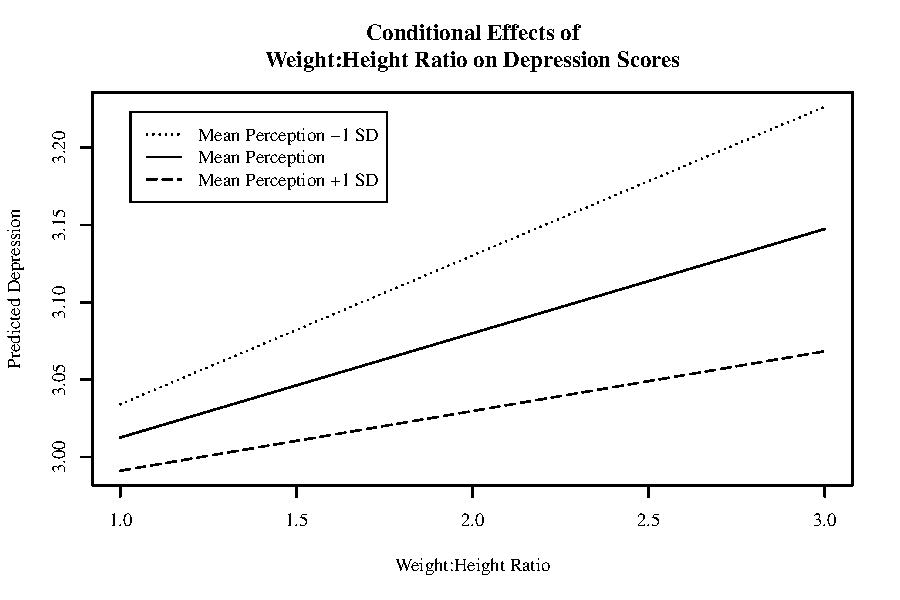
\includegraphics{sweaveFiles/-006}

\end{frame}



\begin{frame}{Probing the Interaction}

  A significant estimate of $\beta_3$ tells us that the effect of $X$
  on $Y$ depends on the level of $Z$, but nothing more.\\
  \va
  The plot on the previous slide gives a descriptive illustration of the
  pattern, but does not support statistical inference.
  \vb
  \begin{itemize}
  \item The three conditional effects we plotted look different, but
    we cannot say that they differ in any meaningful way by only the
    plot and $\hat{\beta}_3$.
  \end{itemize}
  \va
  This is the purpose of \emph{probing} the interaction.
  \vb
  \begin{itemize}
  \item Try to isolate areas of $Z$'s distribution in which
      $\hat{\beta}_3$ is significant and areas where it is not.
  \end{itemize}

\end{frame}


\begin{frame}{Probing the Interaction}

  The most popular approach to probing the interaction is the
  \emph{pick-a-point} approach AKA \emph{simple slopes analysis} or
  \emph{spotlight analysis}.\\
  \va
  The pick-a-point approach tests if the slopes of the conditional
  effects plotted above are
  significantly different from zero.\\
  \va
  To do so, pick-a-point tests the significance of \emph{simple
    slopes}.

\end{frame}


\begin{frame}{Simple Slopes}

  Recall the derivation of our moderated equation:
  \begin{align*}
    Y = \alpha + \beta_1X + \beta_2Z + \beta_3XZ + e_i
  \end{align*}
  We can reverse the process by factoring out $X$ and reordering terms
  to get back to:
  \begin{align*}
    Y = \alpha + (\beta_1 + \beta_3Z)X + \beta_2Z + e_i
  \end{align*}
  Where $f(Z) = \beta_1 + \beta_3Z$ is the linear function that shows
  how the relationship between $X$ and $Y$ changes as a function of
  $Z$.\\
  \va
  \underline{$f(Z)$ is actually our \emph{simple slope}.}
  \vb
  \begin{itemize}
  \item By plugging different values of $Z$ into $f(Z)$, we get the
    slope of the conditional effect of $X$ on $Y$ at the chosen
    value of $Z$.
  \end{itemize}

\end{frame}


\begin{frame}{Significance Testing of Simple Slopes}

  The conditional values of $Z$ used to define the simple slopes in
  the pick-a-point approach are totally arbitrary
  \vb
  \begin{itemize}
  \item The most popular choice is: $\left\{ (\bar{Z} - SD_Z), \bar{Z},
    (\bar{Z} + SD_Z) \right\}$
    \vc
  \item You could also use interesting percentiles of $Z$'s
    distribution
  \end{itemize}
  \va
  The standard error of a simple slope is given by:
  \begin{align}
    SE_{SS} = \sqrt{SE_{\beta_1}^2 + 2Z \cdot \text{COV}(\beta_1, \beta_3) + Z^2 SE_{\beta_3}^2}
  \end{align}
  So, you can test the significance of a simple slope by constructing
  a Wald statistic or confidence interval using $SE_{SS}$:
  \begin{align*}
    Wald_{SS} &= \frac{\hat{f}(Z)}{SE_{SS}}\\
    95\% CI_{SS} &= \hat{f}(Z) \pm 1.96 \cdot SE_{SS}
  \end{align*}

\end{frame}


\begin{frame}[allowframebreaks]{Example}

\begin{Schunk}
\begin{Sinput}
 mod3 <- "
 fX =~ x1 + x2 + x3
 fZ =~ z1 + z2 + z3
 fY =~ y1 + y2 + y3
 fXZ =~ x1z1R + x1z2R + x1z3R +
 x2z1R + x2z2R + x2z3R +
 x3z1R + x3z2R + x3z3R
 
 fY ~ fX + fZ + fXZ
 
 fX ~~ fZ
 fX ~~ 0*fXZ
 fZ ~~ 0*fXZ
 
 x1z1R ~~ x1z2R + x1z3R + x2z1R + x3z1R
 x1z2R ~~ x1z3R + x2z2R + x3z2R
 x1z3R ~~ x2z3R + x3z3R
 
 x2z1R ~~ x2z2R + x2z3R + x3z1R
 x2z2R ~~ x2z3R + x3z2R
 x2z3R ~~ x3z3R
 
 x3z1R ~~ x3z2R + x3z3R
 x3z2R ~~ x3z3R
 "
 out3 <- sem(mod3, data = dat2, std.lv = TRUE)
 summary(out3)
\end{Sinput}
\begin{Soutput}
lavaan (0.5-20) converged normally after  53 iterations

  Number of observations                           500

  Estimator                                         ML
  Minimum Function Test Statistic               74.899
  Degrees of freedom                               113
  P-value (Chi-square)                           0.998

Parameter Estimates:

  Information                                 Expected
  Standard Errors                             Standard

Latent Variables:
                   Estimate  Std.Err  Z-value  P(>|z|)
  fX =~                                               
    x1                0.670    0.043   15.424    0.000
    x2                0.660    0.043   15.256    0.000
    x3                0.704    0.045   15.569    0.000
  fZ =~                                               
    z1                0.738    0.048   15.342    0.000
    z2                0.734    0.048   15.156    0.000
    z3                0.718    0.046   15.602    0.000
  fY =~                                               
    y1                0.396    0.046    8.545    0.000
    y2                0.369    0.044    8.441    0.000
    y3                0.383    0.045    8.558    0.000
  fXZ =~                                              
    x1z1R             0.361    0.053    6.833    0.000
    x1z2R             0.427    0.056    7.615    0.000
    x1z3R             0.432    0.053    8.190    0.000
    x2z1R             0.558    0.056    9.914    0.000
    x2z2R             0.616    0.062   10.008    0.000
    x2z3R             0.520    0.057    9.153    0.000
    x3z1R             0.516    0.059    8.805    0.000
    x3z2R             0.626    0.063   10.007    0.000
    x3z3R             0.521    0.058    8.936    0.000

Regressions:
                   Estimate  Std.Err  Z-value  P(>|z|)
  fY ~                                                
    fX                1.658    0.239    6.930    0.000
    fZ               -0.074    0.099   -0.750    0.453
    fXZ               0.488    0.120    4.049    0.000

Covariances:
                   Estimate  Std.Err  Z-value  P(>|z|)
  fX ~~                                               
    fZ                0.232    0.058    3.987    0.000
    fXZ               0.000                           
  fZ ~~                                               
    fXZ               0.000                           
  x1z1R ~~                                            
    x1z2R             0.273    0.032    8.397    0.000
    x1z3R             0.309    0.033    9.358    0.000
    x2z1R             0.232    0.031    7.566    0.000
    x3z1R             0.235    0.032    7.376    0.000
  x1z2R ~~                                            
    x1z3R             0.231    0.032    7.243    0.000
    x2z2R             0.211    0.035    5.982    0.000
    x3z2R             0.250    0.041    6.163    0.000
  x1z3R ~~                                            
    x2z3R             0.213    0.030    7.010    0.000
    x3z3R             0.213    0.034    6.312    0.000
  x2z1R ~~                                            
    x2z2R             0.247    0.043    5.787    0.000
    x2z3R             0.252    0.040    6.368    0.000
    x3z1R             0.233    0.033    7.103    0.000
  x2z2R ~~                                            
    x2z3R             0.304    0.043    7.086    0.000
    x3z2R             0.199    0.040    5.018    0.000
  x2z3R ~~                                            
    x3z3R             0.139    0.030    4.570    0.000
  x3z1R ~~                                            
    x3z2R             0.212    0.041    5.116    0.000
    x3z3R             0.260    0.040    6.454    0.000
  x3z2R ~~                                            
    x3z3R             0.157    0.041    3.846    0.000

Variances:
                   Estimate  Std.Err  Z-value  P(>|z|)
    x1                0.511    0.042   12.093    0.000
    x2                0.514    0.042   12.221    0.000
    x3                0.548    0.046   11.977    0.000
    z1                0.523    0.052   10.142    0.000
    z2                0.546    0.052   10.444    0.000
    z3                0.461    0.048    9.704    0.000
    y1                0.495    0.043   11.398    0.000
    y2                0.542    0.044   12.334    0.000
    y3                0.444    0.040   11.179    0.000
    x1z1R             0.743    0.050   14.912    0.000
    x1z2R             0.754    0.055   13.682    0.000
    x1z3R             0.694    0.050   13.824    0.000
    x2z1R             0.641    0.057   11.332    0.000
    x2z2R             0.708    0.067   10.575    0.000
    x2z3R             0.671    0.056   12.009    0.000
    x3z1R             0.736    0.060   12.310    0.000
    x3z2R             0.724    0.070   10.277    0.000
    x3z3R             0.707    0.060   11.823    0.000
    fX                1.000                           
    fZ                1.000                           
    fY                1.000                           
    fXZ               1.000                           
\end{Soutput}
\end{Schunk}

\pagebreak
\begin{Schunk}
\begin{Sinput}
 parameterEstimates(out2.1, boot = bootType)[ , -c(1 : 3)]
\end{Sinput}
\begin{Soutput}
     label    est    se      z pvalue ci.lower ci.upper
1       b1 -0.008 0.145 -0.052  0.959   -0.286    0.275
2       b2  0.595 0.142  4.184  0.000    0.317    0.861
3       cp  0.134 0.076  1.763  0.078   -0.019    0.281
4      d21 -0.301 0.110 -2.733  0.006   -0.508   -0.076
5       a2  0.090 0.072  1.253  0.210   -0.073    0.220
6       a1 -0.266 0.061 -4.384  0.000   -0.384   -0.148
7           0.987 0.164  6.013  0.000    0.733    1.390
8           0.689 0.094  7.309  0.000    0.537    0.919
9           0.719 0.112  6.389  0.000    0.535    0.980
10          2.444 0.000     NA     NA    2.444    2.444
11     ab1  0.002 0.040  0.050  0.960   -0.080    0.081
12     ab2  0.053 0.044  1.215  0.225   -0.031    0.146
13  fullIE  0.048 0.026  1.822  0.068    0.012    0.117
14 totalIE  0.103 0.048  2.145  0.032    0.011    0.202
\end{Soutput}
\end{Schunk}

\pagebreak
\begin{Schunk}
\begin{Sinput}
 ## Possible range of a:
 aMarg <- sqrt(s2M * s2Y - sYM^2) * sqrt(s2X * s2Y - sYX^2)
 aInt <- c(
     (sYM * sYX - aMarg) / (s2X * s2Y),
     (sYM * sYX + aMarg) / (s2X * s2Y)
 )
 aInt
\end{Sinput}
\begin{Soutput}
[1] -0.4378558  0.5793099
\end{Soutput}
\begin{Sinput}
 ##
 ## Possible range of b:
 bMarg <- sqrt(s2X * s2Y - sYX^2) / sqrt(s2X * s2M - sMX^2)
 bInt <- c(-1 * bMarg, bMarg)
 bInt
\end{Sinput}
\begin{Soutput}
[1] -1.289996  1.289996
\end{Soutput}
\begin{Sinput}
 ##
 ## max(a):
 aMax <- ifelse(coef(out2)["a"] < 0,
                aInt[1],
                aInt[2])
 aMax
\end{Sinput}
\begin{Soutput}
        a 
0.5793099 
\end{Soutput}
\begin{Sinput}
 ##
 ## max(b)
 bMax <- ifelse(coef(out2)["b"] < 0,
                bInt[1],
                bInt[2])
 bMax
\end{Sinput}
\begin{Soutput}
       b 
1.289996 
\end{Soutput}
\begin{Sinput}
 ##
 ## max(ab)
 abMax <- aMax * bMax
 abMax
\end{Sinput}
\begin{Soutput}
        a 
0.7473075 
\end{Soutput}
\begin{Sinput}
 ##
 ## Kappa Squared:
 k2 <- ab / abMax
 k2
\end{Sinput}
\begin{Soutput}
        a 
0.1359491 
\end{Soutput}
\end{Schunk}


\end{frame}


\end{document}
